\textbf{Pour cette première partie, aucune justification n'est demandée et une seule réponse est possible par question. Pour chaque question, reporter son numéro sur la copie et indiquer la réponse.}

Une réponse fausse ou l'absence de réponse n'enlève aucun point.

\subsection*{Question 1}

Un élève a obtenu les notes suivantes : 11 ; 12 ; 15 ; 9 ; 17 ; 9 ; 8.

La médiane de ses notes est :

\medskip
\begin{tblr}{colspec = {@{}*{4}{X}}}
	\textbf{A.}\quad 9 &
	\textbf{B.}\quad 11 &
	\textbf{C.}\quad 81 &
	\textbf{D.}\quad 12 \\
\end{tblr}

\subsection*{Question 2}

\begin{minipage}[t]{0.6\linewidth}
	La fonction affine $f$ représentée ci-contre a pour expression :

	\medskip
	\begin{tblr}{colspec = {@{}X}}
		\textbf{A.}\quad $f(x) = 2x+6$ \\
		\textbf{B.}\quad $f(x) = -2x+6$ \\
		\textbf{C.}\quad $f(x) = 6x+2$ \\
		\textbf{D.}\quad $f(x) = -3x+6$ \\
	\end{tblr}
\end{minipage}
\hfill
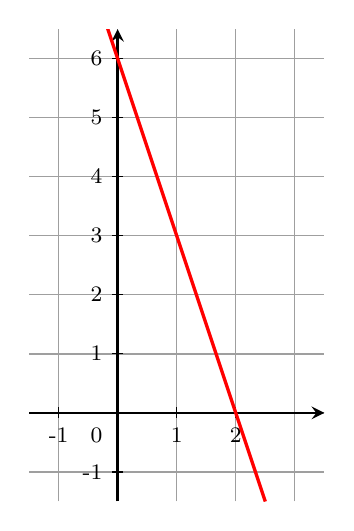
\begin{tikzpicture}[x=0.75cm,y=0.75cm,>=stealth,baseline={(current bounding box.north)}]
	\draw[step=1,gray!75,line width=0.5pt] (-1.5,-1.5) grid (3.5,6.5);
	\draw[->,line width=1pt] (-1.5,0) -- (3.5,0);
	\draw[->,line width=1pt] (0,-1.5) -- (0,6.5);
	\foreach \x in {-1,1,2} \draw (\x,2pt) -- (\x,-2pt) node[below] {\footnotesize \np{\x}};
	\foreach \y in {-1,1,2,3,4,5,6} \draw (2pt,\y) -- (-2pt,\y) node[left] {\footnotesize \np{\y}};
	\draw (-2pt,-2pt) node[below left] {\footnotesize 0};
	\clip (-1.5,-1.5) rectangle (3.5,6.5);
	\draw[line width=1.2pt,red] plot[domain=-0.5:2.5] (\x,{-3*\x+6});
\end{tikzpicture}

\subsection*{Question 3}

L'expression $x^2 - 9$ correspond au développement de :

\medskip
\begin{tblr}{colspec = {@{}*{4}{X}}}
	\textbf{A.}\quad $(x-3)^2$ &
	\textbf{B.}\quad $(x-3)(x+3)$ &
	\textbf{C.}\quad $9(x-1)^2$ &
	\textbf{D.}\quad $(x-9)(x+1)$ \\
\end{tblr}

\subsection*{Question 4}

30\,\% de 12 est égal à :

\medskip
\begin{tblr}{colspec = {@{}*{4}{X}}}
	\textbf{A.}\quad 3,6 &
	\textbf{B.}\quad 36 &
	\textbf{C.}\quad 4 &
	\textbf{D.}\quad 6 \\
\end{tblr}

\subsection*{Question 5}

L'expression $A = \dfrac{\frac{3}{7}}{\frac{4}{5}}$ est égale à :

\medskip
\begin{tblr}{colspec = {@{}*{4}{X}}}
	\textbf{A.}\quad $\dfrac{12}{35}$ &
	\textbf{B.}\quad $\dfrac{15}{32}$ &
	\textbf{C.}\quad $\dfrac{15}{28}$ &
	\textbf{D.}\quad $\dfrac{28}{15}$ \\
\end{tblr}

\subsection*{Question 6}

Sachant que 1 mètre correspond à environ 1,1 yard, 300 mètres représentent environ :

\medskip
\begin{tblr}{colspec = {@{}*{4}{X}}}
	\textbf{A.}\quad 270 yards &
	\textbf{B.}\quad 303 yards &
	\textbf{C.}\quad 330 yards &
	\textbf{D.}\quad 333 yards \\
\end{tblr}

\subsection*{Question 7}

Le nombre $2 \times 2^5$ est égal à :

\medskip
\begin{tblr}{colspec = {@{}*{4}{X}}}
	\textbf{A.}\quad $4^5$ &
	\textbf{B.}\quad $2^{10}$ &
	\textbf{C.}\quad $4^{10}$ &
	\textbf{D.}\quad $2^6$ \\
\end{tblr}

\subsection*{Question 8}

On note $T_F$ la température en degrés Fahrenheit et $T_C$ la température en degrés Celsius.

On a la relation : $T_F = 1,8\,T_C + 32$.

Si la température $T_C$ est de $-10$~\textdegree C, quelle est la température en degrés Fahrenheit ?

\medskip
\begin{tblr}{colspec = {@{}*{4}{X}}}
	\textbf{A.}\quad 30,2 &
	\textbf{B.}\quad 14 &
	\textbf{C.}\quad 50 &
	\textbf{D.}\quad $-50$ \\
\end{tblr}
